\chapter[Indian Renaissance — a Birth \& a Death]{Indian Renaissance — a Birth \&\break a Death}\label{chapter\thechapter:begin}

\Authorline{Manjushree Hegde\footnote{pp.~\pageref{chapter\thechapter:begin}--\pageref{chapter\thechapter:end}. In: Kannan, K S (Ed.) (2018) {\sl Śāstra-s Through the Lens of Western Indology - A Response}. Chennai: Infinity Foundation India.}}
\lhead[\small\thepage\quad Manjushree Hegde]{}

\rhead[]{\small \thechapter. Indian Renaissance — a Birth \& a Death\quad \thepage}

\smallskip
\section*{Abstract}
\smallskip

Sheldon Pollock’s\index{Sheldon Pollock’s} international collaborative project viz. {\sl Sanskrit Knowledge Systems on the Eve of Colonialism} (SKSEC)\index{SKSEC} aspires to trace the intellectual history\index{intellectual history} of pre-modern India\index{pre-modern India} in order to gather a “clearer picture” of the professed death of Sanskrit\index{death of Sanskrit} “in the face of European modernity”. Superficially, SKSEC demonstrates a spirit of openness towards the multiplicity of possible answers to the complex questions it raises. Yet, a closer reading shows that SKSEC works within a fixed framework of predetermined conjectures \& conclusions, and to these, I wish to draw the readers’ attention. 

Firstly, it does not appear to be a strictly construed “intellectual history” that Pollock commits to chart — it appears he is simply enamored by the catch-phrase “{\sl navya}”\index{navya@\textsl{navya}} that was in vogue during the period under examination, and merely wishes to understand what of the {\sl navya}-movement was, in fact, “new”. For Pollock, this word, “{\sl navya}”, is a precious discovery; what he wishes to do with it is to tune the Indian intellectual trajectory into perfect symphony with the European Renaissance\index{Renaissance} — in other words, to equate “{\sl navya}” with “rebirth”/“renaissance”. Further, if Europe\index{Europe} embraced/encouraged the Renaissance, Pollock writes that India largely repudiated the {\sl navya} impulse. Therefore, to Pollock, it was the presence of “something internal, not external, to the Sanskrit\index{Sanskrit} intellectual formation… that arrested the capacity for development by cordoning off the kind of critique that had once supplied that formation’s very life force.”
It is rather clear, then, that SKSEC works on a few presumptions—   
\begin{itemize}
\itemsep=1pt
\item[(a)] that the seventeenth-century Indian intellectual tradition\index{seventeenth-century Indian intellectual tradition} was characterized by certain peculiarities that were comparable to the European Renaissance;

\item[(b)] that they proved completely powerless in the face of their European counterparts, and the millennia-old systems of thought were finally, irrevocably, replaced by the latter; and 

\item[(c)] that an intimate relationship is deducible between Muslim rule\index{Muslim rule} and the avowed “creative upsurge”\index{creative upsurge} of seventeenth-century Indian science.
\end{itemize}

It is a shockingly mischievous endeavor, and I wish to explore the perils of the same.  In the present paper, I examine carefully Pollock’s idea of the “new” in seventeenth-century Indian knowledge systems, their colonial encounter,\index{colonial encounter} and the dubious inferences they lead to.\\[-20pt]

\section*{Introduction}

Sheldon Pollock’s international collaborative project, {\sl Sanskrit Knowledge Systems on the Eve of Colonialism} (SKSEC), is a rather ambitious undertaking. It aspires to trace the intellectual history of pre-modern India in order to gather a “clearer picture” of the professed death of Sanskrit “in the face of European modernity”. 

Intellectual history is an uncharted territory in Indology\index{Indology} — to be sure, it is relatively new to European studies\index{European studies} itself. In general, intellectual history is defined as the study of ideas and intellectual patterns over time, not to be confused with ‘history of ideas’.\index{history of ideas} Peter Gordon,\index{Peter Gordon} an intellectual historian, writes, 
\begin{myquote}
“One thing to note right off is the distinction between “intellectual history” and “the history of ideas”… “history of ideas” is a discipline which looks at large-scale concepts as they appear and transform over the course of history. An historian of ideas will tend to organize the historical narrative around one major idea and will then follow the development or metamorphosis of that idea as it manifests itself in different contexts and times, rather as a musicologist might trace a theme and all of its variations throughout the length of a symphony.” 

\hfill{Gordon (2012:1).}
\end{myquote}

Intellectual history, on the other hand, starts out with the  {\sl a priori} that ideas are “historically conditioned features of the world which are best understood within some larger context”  (Gordon 2012:1). Consequently, it attempts to study ideas in relation to the prevailing social/political/institutional changes of their time. 

Pollock conceived of SKSEC to sketch the ebb and flow of ideas in pre-modern India — because, in his words, “we cannot know how colonialism\index{colonialism} changed South Asia\index{South Asia} if we do not know what was there to be changed” (Pollock 2004:i). Superficially, SKSEC demonstrates a spirit of openness towards the multiplicity of possible answers to the complex questions it raises; Pollock states, in fact, explicitly and repeatedly so, that he only wants to “open up a conversation” on the issue. Yet, a closer reading shows that SKSEC works within a fixed framework of predetermined conjectures and conclusions, and to these, I wish to draw the readers’ attention. 

Firstly, it does not appear to be a strictly construed “intellectual history” that Pollock commits to chart — it is as though he is simply enamored by the catch-phrase “{\sl navya}” that was in vogue during the period under examination (viz. 1550-1750 C.E), and merely wishes to understand what of the {\sl Navya}-movement was, in fact, “{\sl navya}” or “new”. For Pollock, this word, “{\sl navya}”, is a precious discovery; what he wishes to do with it is to tune the Indian intellectual trajectory into perfect symphony with European Renaissance — in other words, to equate “{\sl navya}” with “rebirth”/“renaissance” (Pollock 2000:3)\endnote{This document is available at \url{http://dsal.uchicago.edu/sanskrit/papers/Indian_Knowledge_Systems.pdf}. Document not paginated. One can reach the quote at page no. 3 counting manually.} So, this undertaking tries to identify the characteristics that defined European Renaissance — subjectivity\index{subjectivity}/individuality,\index{individuality} historical awareness,\index{historical awareness} renewed interest in classical texts,\index{classical texts} etc — in the Indian intellectual landscape of the period 1550-1750. Moreover, he aims to attribute this general atmosphere of intellectual dynamism\index{intellectual dynamism} to the consolidation of Muslim rule in India (Pollock 2007: 8).

\newpage

Furthermore, if Europe embraced/encouraged the Renaissance, Pollock writes, India largely repudiated the {\sl navya} impulse. A comparison between the two traditions,\index{traditions} he notes, would show “how differently India and Europe responded to similar conceptual challenges – and how radically, after centuries of homomorphism,\index{homomorphism} their intellectual histories diverged” (Pollock 2007:8). So, according to him, the two traditions — European and Indian — finally differed in how they reacted to this impulse of “newness”\index{newness} and in it lay their respective triumph and downfall (Pollock 2007:8). Therefore, to Pollock, it was the presence of “something internal, not external, to the Sanskrit intellectual formation… that arrested the capacity for development by cordoning off the kind of critique that had once supplied that formation’s very life force” (Pollock 2007:8). It is no wonder, to Pollock, then, that “before the uncompromising modernity that developed in Europe and was disseminated by colonialism, Sanskrit intellectual formation melted like so much snow in the light of a brilliant, pitiless sun.” (Pollock 2000:20)

It is rather clear, then, that SKSEC works on a few presumptions— that, 
\begin{itemize}
\itemsep=1pt
\item[(a)] seventeenth-century Indian intellectual tradition\index{Indian intellectual tradition} was characterized by certain peculiarities that were comparable to the European Renaissance;

\item[(b)] they proved completely powerless in the face of their European counterparts, and the millennia-old systems of thought were finally, irrevocably, replaced by the latter; 

\item[(c)] an intimate relationship is deducible between Muslim rule and the avowed “creative upsurge” of seventeenth-century Indian science (Pollock 2007: 8).
\end{itemize}

In the present paper, I examine carefully Pollock’s idea of the “new” in seventeenth-century Indian knowledge systems, their colonial encounter, and the dubious inferences they allude to.

\newpage

\section{Indian intellectual traditions in the\newline seventeenth-century}

If Pollock wishes to study the seventeenth-century Indian intellectual tradition against the background of the European Renaissance, it would be useful to understand better the latter first. 

Commonly, the Renaissance is understood as a profound transformation of European culture, politics, art and society in the years 1400 C.E – 1600 C.E.  It describes both a period in history and a more general ideal of cultural renewal. ‘{\em Renaissance}’, in French, literally means “rebirth”. To Jules Michelet,\index{Jules Michelet} the first person to use this term (in the 19$^{\rm th}$ century), the word meant, “…the discovery of the world and the discovery of man..” (Brotton 2006:10) 

Michelet was the first to define the Renaissance as a definitive historical moment that disassociated itself from the Middle Ages;\index{Middle Ages} furthermore, he was the first to promote it as a particular “spirit” or “attitude”, rather than simply a specific historical period. For him, this period, in general, represented a progressive, democratic worldview that celebrated the virtues he valued— Reason, Truth, Art,\index{Art} and Beauty. According to Michelet, the Renaissance “recognized itself as identical at heart with the modern age” (Brotton 2006:10).

It is worth quoting the long message of Brotton: 
\begin{myquote} 
“Michelet’s Renaissance does not happen in Italy in the 14th and 15th centuries, as we have come to expect. Instead, his Renaissance takes place in the 16th century. As a French nationalist, Michelet was eager to claim the Renaissance as a French phenomenon. As a republican, he also rejected what he saw as 14th-century Italy’s admiration for church and political tyranny as deeply undemocratic, and hence not part of the spirit of the Renaissance. Michelet’s story of the Renaissance was shaped decisively by his own 19th-century circumstances. In fact, the values of Michelet’s Renaissance sound strikingly close to those of his cherished French Revolution:\index{French Revolution} espousing the values of freedom, reason, and democracy, rejecting political and religious tyranny, and enshrining the spirit of freedom and the dignity of ‘man’. Disappointed in the failure of these values in his own time, Michelet went in search of a historical moment where the values of liberty and egalitarianism triumphed and promised a modern world free of tyranny.”	\hfill{Brotton (2006: 11)}
\end{myquote}

\newpage

If Michelet fashioned the idea of Renaissance, it was Jacob Burckhardt\index{Jacob Burckhardt} who defined it as a 15th-century Italian (not French) phenomenon. In 1860, Burckhardt published his work, {\sl The Civilization of the Renaissance in Italy}. In it, he argued that it was the peculiarities of political life in late 15$^{\rm th}$ century Italy that led to the creation of a “recognizably modern individuality”. Accordingly, the revival of classical antiquity, the discovery of the wider world, and the growing unease with organized religion meant that “man became a spiritual individual.” Burckhardt contrasted this with the lack of individual awareness that for him defined the Middle Ages—  “…(in the middle ages) man was conscious of himself only as a member of a race, people, party, family or corporation” (Brotton 2006: 11). Brotton writes,
\begin{myquote}
“Burckhardt says very little about Renaissance art or economic changes, and overestimates what he sees as the skeptical, even ‘pagan’ approach to religion of the day. His focus is exclusively on Italy; he makes no attempt to see the Renaissance in relation to other cultures. His understanding of the terms ‘individuality’ and ‘modern’ also remain extremely vague. Like Michelet, Burckhardt’s vision of the Renaissance reads like a version of his own personal circumstances.”  

\hfill{Brotton (2006: 12)}
\end{myquote}

Michelet and Burckhardt’s celebrations of art and individuality found their logical conclusion in Walter Pater’s\index{Walter Pater} work, {\sl The Renaissance}. Rejecting the political, scientific, and economic aspects of the Renaissance, Pater saw only “a spirit of rebellion and revolt against the moral and religious ideas of the time” in the art of 15th century works, and therefore, wrote of “the love of art for its own sake”. It was a hedonistic celebration of what Pater called “the pleasures of the senses and the imagination”.  

So it was that Michelet, Burckhardt, and Pater created an idea of the “spirit of Renaissance”. It is not an accurate historical account of what took place in 15th century Europe — it simply captures an ideal of the later society. 

If the Renaissance did not occur even in Europe in the way it is imagined, and showcased to be, it seems rather pointless to demonstrate an “Indian Renaissance”, and draw parallels between the two “movements”. Yet, that is precisely what Sheldon Pollock sets out to do. 

\newpage

In his project SKSEC, he starts with a questionable {\sl a priori} that the two centuries (1550-1750) – just prior to the colonial encounter – witnessed an unprecedented “flowering of intellectual life” in India — remarkably comparable with European Renaissance. A significant number of SKSEC’s working-papers are, in fact, committed to finding the same novelty in seventeenth-century Indian intellectual traditions. Let us, then, examine the “newness”/distinguishing characteristics of seventeenth-century Indian knowledge systems as purported by Sheldon Pollock.

\subsection{Upsurge in writing}%%%1.1

\vskip -.25cm

One of the characteristic features of pre-colonial\index{pre-colonial} Indian science, according to Pollock, is the “explosion of scholarly production” beginning in the 16$^{\rm th}$ century. According to him, an extraordinary upsurge in writing — previously unmatched — occurred across intellectual disciplines in this period. It is comparable, he says, to the renewed interest in the classical disciplines of the Renaissance. 

It must be noted here that Pollock chooses to examine only those disciplines where he is likely to find the said “upsurge in writing”; and in those where he sees no such trend, he chooses to reject them in favor of the others.

Furthermore, for Pollock, this trend is no mere artefact of preservation. According to him, there is absolutely no evidence to show that anything substantial was lost in the preceding period. He cites the example of Caṇḍeśvara’s work in political theory to validate his point — Caṇḍeśvara,\index{Candesvara@Caṇḍeśvara} apparently, refers to only one text from the entire preceding two centuries, and therefore, Pollock concludes, “the upsurge we see is real” Pollock (2007: 8).

Below is a statistical analysis of all the available works (of three disciplines viz. Pūrvamīmāṁsā,\index{Purvamimamsa@Pūrvamīmāṁsā} Vedānta\index{Vedanta@Vedānta} and Nyāya\index{Nyaya@Nyāya}) through the centuries. It is based on Karl. H. Potter’s (2009-2015) encyclopedia of Indian philosophical systems, and approaches near accuracy. If proliferation of texts — or their availability, discounting any loss of material — is a measure of a knowledge-system’s status, may we safely conclude that Pūrvamīmāṁsā is vigorously alive — in fact, almost at its zenith — today?   

\newpage

\begin{landscape}
~\phantom{a}
\vfill
\begin{figure}[H]
\centering
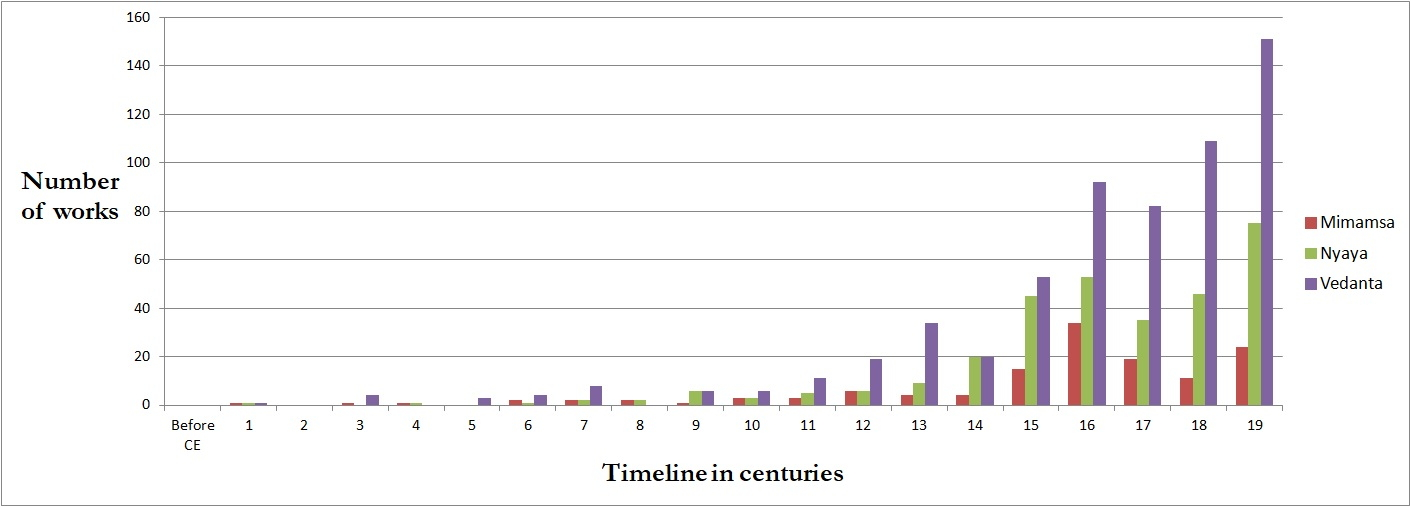
\includegraphics[scale=1.4]{figures/fig1.jpg}
\caption{Number of (extant) texts of Indian Knowledge Systems (100 CE - 1900 CE)}\label{chap2-fig1}
\end{figure}
\vfill
~\phantom{a}
\end{landscape}

\eject

If, on the other hand, we ignore the minor works, and make a list of only the prominent writers of a discipline, we find a table of a different sort: 
\begin{table}[H]
\centering
\tabcolsep=3pt
\renewcommand{\arraystretch}{1.2}
\begin{tabular}{|l|l|l|l|}
\hline
\textbf{Time-period} & \textbf{Vyākaraṇa}\index{Vyakarana@Vyākaraṇa} & \textbf{Mīmāṁsa} & \textbf{Nyāya-Vaiṣeśika}\index{Nyaya-Vaisesika@Nyāya-Vaiṣeśika}\\\hline
5th B.C & Pāṇini &  Jaimini  & \\\hline
& Yāska & & \\\hline
4th B.C & Vyāḍi & & \\\hline
& Vājapyāyana & & \\\hline
3rd B.C & Kātyāyana & & \\\hline
2nd B.C & Patañjali\index{Patanjali@Patañjali} & & Kaṇāda\\\hline
2nd C.E & & & Gautama\\\hline
4th C.E & & Śabara & Vātsyāyana\\\hline
5th C.E & Bhartṛhari & & Praśastapāda\\\hline
6th C.E& & & Uddyotakara\\\hline
7th C.E & Vāmana & Kumārila & \\\hline
& Jayāditya & Prabhākara & \\\hline
& & Maṇḍanamiśra & \\\hline
10th C.E & Helarāja & Pārthasārathi & Jayantabhaṭṭa\index{Jayantabhatta@Jayantabhaṭṭa}\\\hline
 & Puṇyarāja & Vacaspati & Śrīdhara\\\hline
11th C.E & & Someśvara & Udayana\\\hline
& & Bhavadeva & \\\hline
12th C.E. & Kaiyaṭa & & Gaṅgeśa\\\hline
15th C.E & & & Raghunātha\\\hline
16th C.E & Bhaṭṭoji Dīkṣita & & Mathuranātha\\\hline
17th C.E & Haridikṣita & Gāgābhaṭṭa & Jagadīśa\\\hline
& Kauṇḍabhaṭṭa & Khaṇḍadeva & Gadādhara\\\hline
& & & Annambhaṭṭa\\\hline
& & & Padmanābhamiśra\\\hline
18th C.E  & Nāgeśa Bhaṭṭa & & \\\hline
\end{tabular}
\caption{Prominent exponents of (three) Indian Knowledge Systems}\label{chap2-tab1}
\end{table}

\newpage

Neither the Figure nor the Table, supports as we can see, Pollock’s flavor of argument in respect of either peaks or troughs.

\subsection{Newness of form}%%% 1.2

Pollock writes that a significant innovation of style is observable in the works of this period – an adoption of the new philosophical meta-language\index{meta-language} characterized by the excessive employment of the highly refined terminologies of Navya-nyāya.\index{Navya-nyaya@Navya-nyāya} This, of course, is true. But it is important to note that this trend was initiated in the thirteenth century itself by Gaṅgeśa\index{Gangesa@Gaṅgeśa} in Mithilā\index{Mithila@Mithilā}. Gaṅgeśa developed the technique of subtle argumentation in his {\sl magnum opus}  viz. {\sl Tattvacintāmaṇi}.\index{Tattvacintamani@\textsl{Tattvacintāmaṇi}} The tradition was carried forward by Vardhamāna (fourteenth century), Yajñapati Upādhyāya (fifteenth century), and Pakṣadhara Miśra (fifteenth century), among others. From Mithilā, Navya-nyāya travelled to Navadvīpa\index{Navadvipa@Navadvīpa} in Bengal.\index{Bengal} Raghunātha Śiromaṇi\index{Raghunatha Siromani@Raghunātha Śiromaṇi} (sixteenth-century) of Navadvīpa wrote a commentary on {\sl Tattvacintāmaṇi} entitled {\sl Dīdhiti}\index{Didhiti@Dīdhiti} in which he introduced a few changes in Navya-nyāya metaphysics and epistemology. Subsequent proponents of Navya-nyāya in Bengal — including Bhavānanda Siddhāntavāgīśa, Mathurānātha Tarkavāgīśa, Jagadīśa Tarkālaṅkāra and Gadādhara Bhaṭṭācārya — wrote commentaries on {\sl Dīdhiti} which contributed to the fullest development of Gaṅgeśa’s technique of reasoning. 

The fame of Navadvīpa {\sl naiyāyika}-s\index{naiyayika@\textsl{naiyāyika}} spread all over India, and scholars from other schools adopted the Navya-nyāya language.  Irrespective of the ontological, epistemological, and moral commitments of the discussants, this highly technical language became the medium for all serious philosophical discussion by the sixteenth century — primarily because of its ontological neutrality. Navya-nyāya style, it may be conjectured, is not intended for the purpose of communicating more easily, any more than the mathematicians’ is; it is intended rather to provide an accurate framework for the presentation of the world as it really is. If seventeenth-century India saw an extraordinary spread of the use of Navya-nyāya language, it can only be said to be a natural development of the seeds sown in the thirteenth century. And to attribute this use of Navya-nyāya to Persian-interactions\index{Persian-interactions} of the sixteenth \& seventeenth centuries is a no less than a fanciful stretch of imagination supported by not a shred of proof. 

\subsection{Multidisciplinary pursuits}%%% 1.3

According to Pollock, the sixteenth-seventeenth centuries saw the rise of interdisciplinary pursuits.

 “There is, for one thing, a new multidisciplinarity\index{multidisciplinarity} on the part of scholars. Earlier hermeneutists never wrote juridical treatises (or scholars of jurisprudence hermeneutics), let alone aesthetics; it now became common”\hfill Pollock (2007: 8).

This is a rather sweeping generalization to make — Indian tradition has seen its share of polymaths\index{polymaths} throughout its history: 

To illustrate: (2$^{\rm nd}$ – 1$^{\rm st}$ century BCE) Patañjali  — credited with works on grammar, medicine, and yoga\endnote{The tradition that the same Patañjali wrote treatises on grammar, medicine and yoga is memorialized in a verse by Bhoja in his commentary on the {\sl Yoga-sūtra}-s. Bhoja was perhaps influenced by a verse by Bhartṛhari that speaks of the genesis of the three {\sl śāstra}-s in order to rid one of impurities at the levels of the body, the speech, and the mind viz. {\sl cikitsā} (medicine), {\sl lakṣaṇa} (grammar), and {\sl adhyātma} (spirituality). ({\sl Vākyapadīya} 1.146). Bhoja's verse reads thus: {\sl yogena cittasya padena vācāṁ malaṁ śarīrasya ca vaidyakena} | {\sl yo’pākarot taṁ pravaraṁ munīnāṁ patañjaliṁ prāñjalir ānato’smi} ||;}

\vskip .1cm

(950-1016 CE) Abhinavagupta\index{Abhinavagupta} — credited with works on poetics and Kashmir philosophy; 

(1088 – 1173) Hemacandra\index{Hemacandra} — grammar, philosophy, prosody, history; 

(1010-1055 CE) King Bhoja\index{Bhoja}  — philosophy, poetry, grammar, medicine, veterinary science, phonetics, yoga, archery, etc; 

(960 CE) Vācaspati Misra\index{Vacaspati Misra@Vācaspati Misra}  — six systems of philosophy; 

(ca. 1330 CE) Vedānta Deśika;\index{Vedanta Desika@Vedānta Deśika} 

(ca. 1350 CE) Vidyāranya;\index{Vidyaranya@Vidyāranya} 

(ca. 1450 CE) Mallinātha Sūri\index{Mallinatha Suri@Mallinātha Sūri}

- to name a few. 

\vskip .1cm

Below is a statistical analysis of the scholars who have written at least one work on Pūrvamīmāṁsa/Nyāya, and also on (at least) one other {\sl śāstra}\index{sastra@\textsl{śāstra}} (based, again, on Karl Potter’s Encyclopedia of Indian philosophical systems).\index{Indian philosophical systems} 

Again, if availability of texts, discounting any loss of material, is to be used as a yardstick of the intellectual climate of India, a claim of a sharp rise of multidisciplinary pursuits in exactly the period under examination (viz. 100 CE - 1900 CE) remains an unsubstantiated conjecture.

\newpage

\begin{landscape}
~\phantom{a}
\vfill
%\begin{sidewaysfigure}
\begin{figure}[H]
\centering
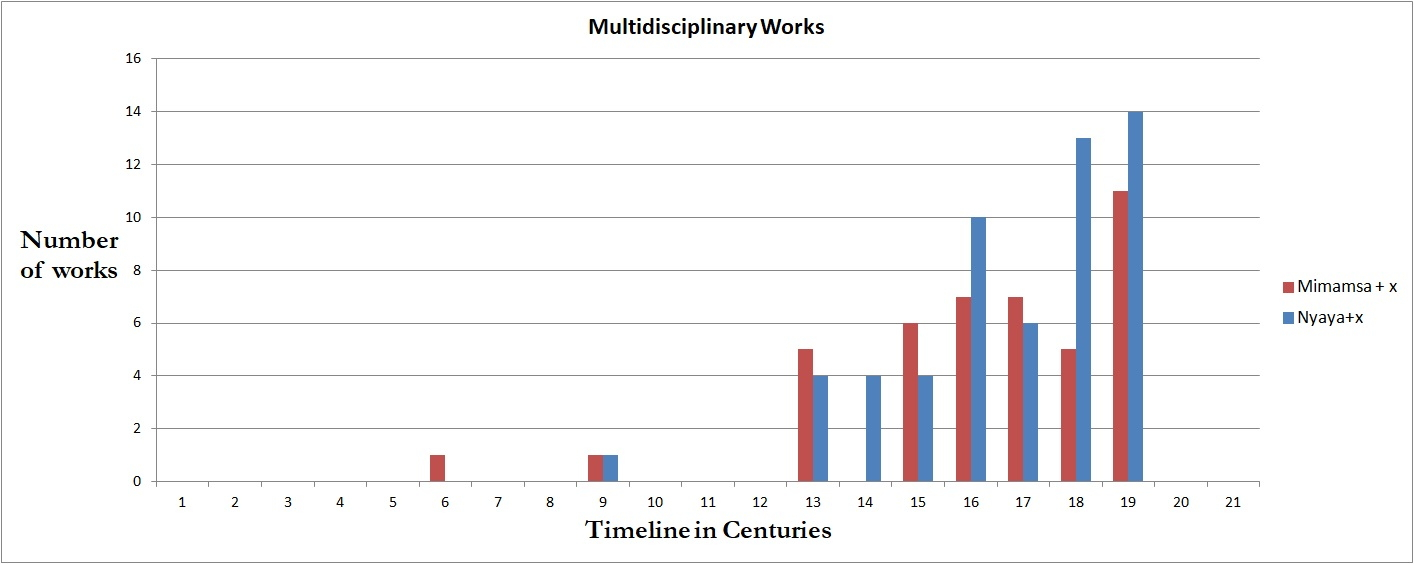
\includegraphics[scale=1.37]{figures/fig2.jpg}
\caption{Number of multi-disciplinary scholars (100 CE - 1900 CE)}\label{chap2-fig2}
%\end{sidewaysfigure}
\end{figure}
\vfill
~\phantom{a}
\end{landscape}

\newpage


\subsection{Subjectivity}%%% 1.4

According to Pollock, the “new cross-cultural interactions…that began to take place from the beginning of the Mughal\index{Mughal} period were without parallel for the conceptual and social distances being bridged, especially among Sanskrit and Persianate intellectuals at the Mughal court” (Pollock 2000:17). 

\vskip .1cm

It must be noted here that Pollock reasserts, in the same breath, that we have only the vaguest notions about the material conditions of life of seventeenth-century Sanskrit intellectuals, their sources of patronage\index{patronage} and relations with courtly power, their networks of intellectual exchange and circulation, about their modes of association or the institutional structures in which they worked, etc. 

\vskip .1cm

For most of the key thinkers in question, he writes, “we are confronted by an absence of contextuality that is almost absolute” (Pollock 2000:4). How he makes the outlandish associations, then, is a matter known only to him. 

\vskip .1cm

He continues: inseparable from the new social circumstances of these scholars was the presence of a “striking new subjectivity” in their literary works (Pollock 2001a:20).  

\begin{myquote}
“Never before in Sanskrit literature had a writer constructed a self quite so vividly present as Siddhichandra does in his autobiography. The work itself, embedded in the biography of his teacher, almost objectifies the tension between a very old conception of heteronomy and a very new self-fashioning that the text treatises throughout. Jagannātha composed verses on the death of his wife that are unprecedented in earlier Sanskrit poetry, and his lyrics on a Yavanī woman he named Lāvaṅgī ({\em sic})\endnote{The name of the lady is Lavaṅgī, not Lāvaṅgī. The oft-quoted verse has ``{\em lavaṅgī kuraṅgīdṛgaṅgīkarotu} (Note that ``{\em lāvaṅgī}'' would violate the metre) (Ref. Durgaprasad and Pansikar 1916: 1)} (who almost certainly had become his wife) are probably an appropriation of the Persian motif of the {\sl mahbūb}, the ever-unattainable beloved whose unattainability is typically exaggerated by the code of the otherness…” 

\hfill Pollock (2001a:20)
\end{myquote}

\vskip .1cm

In every paper on this topic\endnote{Refer these four papers of Pollock (written over 7 years) : Pollock (2003), (2001a), (2001b), (2007).}, Pollock has just these two examples to furnish to substantiate his claim — that of Siddhicandra\index{Siddhicandra} and Jagannātha Paṇḍita.\index{Jagannatha Pandita@Jagannātha Paṇḍita} To be sure, there are a number of anecdotes about Jagannātha Paṇḍita. Of them P.V.\ Kane\index{Kane P.V.} writes, “The story about Jagannātha’s liaison with a Yavana damsel called Lavaṅgī\index{Lavangi@Lavaṅgī} (in such verses as {\sl yavanī navanīta}, etc) appears to be a myth spread by those who were offended by the biting tongue (rather pen) of Jagannātha.” (Kane 1961:324) 

The said verse (that speaks of the loss of a great love) occurs in Jagannātha’s collection of {\sl muktaka}-s (independent verses), entitled {\sl Bhāminī-vilāsa},\index{Bhamini-vilasa@\textsl{Bhāminī-vilāsa}} and is also analyzed in his {\sl Rasa-gaṅgādhara}.\index{Rasa-gangadhara@\textsl{Rasa-gaṅgādhara}} 

This same verse — that to Pollock are the outpourings of a grief-stricken mind— are analyzed in the {\sl Rasa-gaṅgādhara} — by the same author — in an attitude of clinical detachment. When discussing the poem cited above, Jagannātha offers, to cite Pollock’s own words, two possible explanations: 

\begin{myquote}
“This may be spoken by someone absent from home, perhaps a young man who has fallen in love with the beautiful daughter of his teacher while in school, or someone else thinking back on an illicit sexual relationship he has had” 
\hfill (Pollock 2001b: 411) 
\end{myquote}

Similarly, the other poem found in {\sl Karuṇā-vilāsa} — which, according to Pollock, is Jagannātha’s lamentation of the death of his son — is analyzed clinically by Jagannātha in the {\sl Rasa-gaṅgādhara.}

Most easily, the issue is resolved if the {\sl muktaka}-s are not considered as an account of Jagannātha’s life. Yet, it must be remembered that “individuality” was not absolutely absent in earlier works. Indian intellectual landscape is dotted with a healthy dose of chronicles of historical figures — 

Daṇḍin’s {\sl Avantisundarīkathāsāra}, 

Bāṇabhaṭṭa’s {\sl Harṣacarita},

works of Bhavabhūti, 

Kalhaṇa’s {\sl Rājataraṅginī}, 

Vākpati’s {\sl Gauḍavāho}, 

Chand Bardai’s {\sl Prithivīrāj Raso}, 

Bilhaṇa’s {\sl Vikramāṅkadevacarita}, 

Jayānaka’s {\sl Prithivirājavijaya}, 

Vidyācakravartin’s {\sl Gadyakarṇāmṛta}, 

Gaṅgā\-devī’s {\sl Madhurāvijaya}, 

Jayasiṁha’s {\sl Kumārapālacarita}, 

Hemachandra’s {\sl Hammīra-mada-mardana}, 

Ballāla’s {\sl Bhojaprabandha},  to name a few. 

In fact, in Sanskrit poetics, there exists a genre called {\sl ākhyāyikā}\index{akhyayika@\textsl{ākhyāyikā}} that demands the chronicles of factual events. The oldest writer on Poetics who dealt with this matter was Bhāmaha\index{Bhamaha@Bhāmaha} who drew a rigid distinction between the {\sl ākhyāyikā} and the {\sl kathā}\index{katha@\textsl{kathā}} (imaginative fiction). Laying down the definition of an {\sl ākhyāyikā}, Bhāmaha wrote that the former must be a literary composition in which “an account of his own deeds is given by the hero himself”— 

{\sl vṛttam ākhyāyate tasyām nāyakena sva-ceṣṭitam} 	          \hfill{({\sl Kāvyālaṅkara} 25-9)}

Here, the word {\sl vṛtta} in connection with {\sl sva-ceṣṭita} indicates “actual history” or “facts of experience” as opposed to “invented fiction”(cf. the famous definition {\sl kathā kalpita-vṛttāntā, vṛttārthākhyāyikā matā}). Also, we should note the admittedly {\sl a posteriori} nature of this early work on Alaṁkāra — the conclusions were most probably based upon the observance of prevalent works — so, Jagannātha was by no means the first poet to write an account of his own life — if it is admittedly that.  

If Pollock wishes to attribute — this as a characteristic feature of the sixteenth-seventeenth centuries, and also to attribute it to Mughal interactions, he must ground his arguments on more solid facts. Funnily, analyzing the works of two other poets of the period, Pollock contradicts his own words,

 “… that a radical alteration in social environment can fail to produce a commensurate transformation of cultural vision is even more patent in the life of Kavīndrācārya Sarasvatī (ca. 1600–75).” 

\hfill (Pollock 2001a:25)

It would make his case stronger/clearer if only Pollock would decide if or not the “radical alteration in social environment” made a radical transformation of traditional minds!\\[-20pt] 

\subsection{Historicity}%%% 1.5

Yet another distinguishing feature of this period, according to Pollock, is a historical, “perhaps even historicist”, conceptual framework for understanding the development of knowledge systems. With continued regularity, Pollock has but a single example to substantiate his claim in all his papers on the subject\endnote{See Pollock (2000), (2004), and (2001a).} — that of Mahādeva’s\index{Mahadeva@Mahādeva} {\sl Nyāya-kaustubha}.\index{Nyaya-kaustubha@\textsl{Nyāya-kaustubha}} 

Pollock admits that it is unfair to infer from this evidence and his arguments based on it that prior to this period, chronological thinking as such was never attested, that earlier knowledge was never described as earlier in scholarly discourse. It is, after all, a well-known fact that polymaths like Abhinavagupta, Vacaspati Miśra, etc. followed a similar chronological-method of argument. In fact, Vacaspati Miśra (960 C.E) had specifically divided the followers of Prabhākara Miśra into “{\sl Jarat-Prābhākara}-s”, and “{\sl Navya-Prābhākara}-s”.  
\begin{myquote}
“Such is certainly not the case”  “… but what I do wish to suggest is that in the seventeenth century, for the first time, knowledge was believed to be better not just because it might objectively be better — endowed with greater coherence, economy,\index{economy} explanatory power — but also in part because it was new.”  \hfill{Pollock (2001a:11)}
\end{myquote}

Pollock is incorrect. For most later scholars, too, ‘new’ signified ‘anti-traditional’,\index{anti-traditional} and it was usually employed as a term of reproach: Jagannātha, too, for that matter, did not intend to break with the past history of his discipline; we see that he employed his rigorous approach most energetically when combating what he saw as threats to the traditional approaches of poets.

We see here that Sheldon Pollock starts from an {\sl a priori} that Indian intellectual tradition considered “knowledge of every variety … fixed in its dimensions … [and] does not change or grow, but is frozen” and hence “there can be no conception of progress”. Innovations are thus “viewed, through the inverting lens of ideology, as renovation and recovery” of knowledge permanently fixed (Pollock 1985:515).  

But it must be understood that tradition in India, in Coomaraswamy’s\index{Coomaraswamy} words, “has nothing to do with any “ages”, whether “dark”, “primeval”, or otherwise... Tradition represents doctrines about first principles, which do not change; and traditional institutions represent the application of these principles in particular environments… metaphysics is not a system, but a consistent doctrine; it is not merely concerned with conditioned and quantitative experience, but with universal possibility…” (Lipsey: 1987:37). Furthermore, it is unreasonable to view the absence of the idea of new as “progress”\index{progress} in India, as a sign of stagnation; after all, not always is success (as in modernity) the capacity to expand; success is also the capacity to endure. There is no law of chronic deficiency in human affairs mandating that societies, like cities, must always be under construction and never complete, that understandings of literary art, the structure of the moral order, or the organization of power\index{power} can never achieve something like adequacy or even perfection for the social world concerned, but must be constantly rejected for something newer and better - the very slogan of modernity.  

If it were not for the commitment to finding differences, Pollock would see that it is far easier to see the continuity of the tradition than its divergence. In Coomaraswamy’s words, “The passionless reason of its “objective” scholarship, applied to the study of “what men have believed” is only a sort of frivolity, in which the real problem, that of knowing what should be believed, is evaded” (Coomaraswamy 1943:6). In practice, Indian knowledge systems’ capacity to assimilate variation is, in fact, its most salient feature. Broadly viewed, the tradition has retained, right up to modern times, a kind of non-coercive elasticity and expressive virtuosity that have been there all along — in a way, it is precisely this elegant mechanism of continuous cultural self-invention that has allowed it to stay strong in the face of the cultural invasion.\\[-20pt] 


\subsection{Newness of Intellect, Oldness of Will}%%%1.6

In his defense, Pollock does, in fact, recognize the continuity of the tradition; only, he chooses to derogatorily call it an “oldness of will”. We offer here two citations of Pollock in support of our remark.
\begin{myquote}
“He was an “innovative traditionalist,” … for whom the new was “intimately connected to reestablishing the old” – an intellectual objective very widely shared in this epoch, but about whose intellectual-historical, or social-historical, logic we currently understand next to nothing.” \hfill{Pollock (2001a:4)}

\vskip .1cm

“Radically at odds, however, with the genuine innovations signaled by historicist exposition, discursive style, and mode of argument was the traditionalism of the scholarly problematics themselves… The universe of thought, it seems, did not expand in a way at all commensurate with the expansion of the instruments and styles of thought the philosophical question itself, the method of analysis of the problem, and the actual judgment rendered, were archaic…”\hfill{Pollock (2001a:12)}
\end{myquote}
In reaction to Pollock’s conjectures, Brian Hatcher\index{Brian Hatcher} asks aptly, “… in a rather unfortunate bit of metaphorics, Pollock evoked “newness of intellect constrained by an oldness of the will” – as if the appeal to a quasi Augustinian anthropology could do justice to the complexity of the changes he was interested in highlighting… is there a theory here or just flip phraseology?” (Hatcher 2007: 340) 

A more correct explanation of the phenomenon would be that, during the 14$^{\rm th}$-16$^{\rm th}$ century C.E, the original {\sl sūtra}-s\index{sutra@\textsl{sūtra}} and scholia had receded into the background — later texts had become a center for a mass of commentarial literature, a web of complicated meta-linguistic innovations in the search for ever greater precision and sophistication of definition and analysis. Bodas remarks,
\begin{myquote}
“Here we see at one and the same time scholasticism at its climax and true philosophy at its lowest depth. We might wade through volumes of controversial jargon without coming across a single flash of deep thought or real insight into the nature of things. Mere conventionalities and distinctions without a difference are the weapons of this wordy warfare…” \hfill{Bodas (1918:L)}
\end{myquote}

A kind of reaction against the excesses of this scholasticism\index{scholasticism} seems to have led the writers of the seventeenth century to seek fresher insights from the founts of the early {\sl sūtra} literature. Another sign of this reaction was the production of manuals adapted to the understanding of the beginners – the {\sl Bhāṣā-Pariccheda}, {\sl Vedānta-paribhāṣā}, etc are instances of this class of books which must have come as a relief to those students who were hitherto lost in the mazes of {\sl Pañca-lakṣaṇī} and {\sl Advaita-siddhi}. 

Now, if Pūrvamīmāṁsā teaches anything, it is to choose, in Śabara-svāmin’s\index{Sabara@Śabara} words, the {\sl saṁnikṛṣṭārtha} (nearer meaning) over the {\sl viprakṛṣṭārtha} (remote meaning) in the interpretation of texts; and logically, this is the simplest and most reasonable explanation for the “increase in the production of independent treatises and of works that directly comment on ancient foundational ({\sl sūtra}) texts while summarizing the entire earlier history of interpretation, and in the concomitant decrease in ever more deeply nested commentaries on commentaries\index{commentaries} on canonical works that had been a hallmark of the earlier schoolmen” (Pollock 2000:11).

Furthermore, according to Pollock, Europe embraced the “newness” that emerged— this resulted in its modernity/progress; India, on the other hand, remained prude, and the “tension” between the old\index{old} and the new eventually played the key role in Sanskrit’s downfall.

It must be understood here that the production of Western modernity was a response to a set of very peculiar historical circumstances and institutions — none of which were known in India. There was no church\index{church} to produce heresy, ex-communication and censorship or to provoke Reformation,\index{Reformation} Counter-Reformation and religious wars. There was no regime of conquest to promote foreign colonization, and no absolutist state to construct a repressive security apparatus. On the other hand, Sanskrit intellectuals were {\rm radically free}. 

Writing about secularism,\index{secularism} Michel Danino\index{Michel Danino} remarks,
\begin{myquote}
“Secularism was born to challenge theocracy in the Christian and Islamic worlds. In medieval Europe, political power was in almost every country held or at least controlled by one Church or another. It took nearly two centuries, the eighteenth and nineteenth, to curtail that power and establish a complete separation between Church and State—which is what secularism has meant in the West, as any good dictionary will tell us. In France, for instance, the Roman Catholic Church was virtually all-powerful until the French Revolution, and only a century later did it finally lose its control over education. Secularism meant keeping the Church away from political power and from education, it meant a polity free from Christian affiliation. Likewise, when Mustapha Kemal threw out the Sultan in Turkey and established a “secular republic” in 1923, it was because he had abolished the office of the Caliph of the Islamic world; “secularism” to him meant keeping Islam away from political power.  This notion of secularism has no application in India, where theocracy never existed; how could it, in the absence of an organized Church or
clergy? Even so conformist a historian as Vincent Smith noted that: “Hindooism has never produced an exclusive, dominant, orthodox sect, with a formula of faith to be professed or rejected under pain of damnation.”	\hfill{Danino (2005)}
\end{myquote}

In short, it was the absence in India of the miseries of Europe’s peculiar circumstances and institutions that entailed the absence of Europe’s peculiar modernity. If the latter was a mark of freedom, of protest against medieval asceticism and ecclesiastical restraint, if it heralded an intellectual revitalization and thus stirred the universal mind and heart of Europe, in India, this song played not— simply because it was unnecessary. On the other hand, India always was what Europe has somewhat been since Renaissance – with no censorship, no excommunication, and no ecclesiastical restraint.

\subsection{Vernacularization}%%% 1.7

Sheldon Pollock has always expressed a keen interest in the problem of power — more specifically, “in the intermeshing of cultural (literary, scientific, ideological) production with the political domain” (Bronner \& Shulman 2006:13). In his important work, “{\em The Language of the Gods in the World of Men}”,\index{The Language of the Gods in the World of Men@\textsl{The Language of the Gods in the World of Men}} he has written exhaustively on the process of “vernacularization” that, according to him, occurred between ca.1000 and 1500.

One must note here that on the one hand, Pollock insists that in the seventeenth century, an un-mendable cultural split (between Sanskrit and vernacular intellectual worlds) was already in place; yet, on the other hand, he writes that the Sanskrit world crumbled because it did not embrace the vernacularization.\index{vernacularization}

If he is to be believed, Sanskrit simply withered on the branch when “court intellectuals” decided to abandon the global language of Sanskrit and speak locally in their literary and political texts. Here, Shulman\index{Shulman} \& Bronner’s\index{Bronner} work, {\sl A Cloud Turned Goose: Sanskrit in the Vernacular Millennium},\index{A Cloud Turned Goose: Sanskrit in the Vernacular Millennium@\textsl{A Cloud Turned Goose: Sanskrit in the Vernacular Millennium}} is an interesting reference to observe — with the example of Vedānta Deśika’s {\sl Haṁsa Sandeśa},\index{Hamsa Sandesa@\textsl{Haṁsa Sandeśa}} they argue that Sanskrit poetry played a critical — and highly original — role in the {\sl elaboration} of regional cultural identities. Accordingly, Sanskrit, “serving as an available and localized medium in each and every region separately, participated along with the vernaculars in the project of inventing and elaborating distinctive regional cultures and identities. Far from occluding such regional distinctiveness or uniqueness, Sanskrit was now employed precisely to articulate it” (Bronner \& Shulman 2006:6). In their words,
\begin{myquote}
“… Sanskrit still allows a poet to transcend his or her parochial context and reach out to a space shaped by a wider, inherited discourse. At the same time, Sanskrit enables a skilled poet to condense into the space of a single work— even a single verse — an entire world of specific associations, contents and meaning… It is clear, at least to me, that Sanskrit did not share Latin’s fate. Intense regionalization in the literary realm tended to go hand in hand with highly innovative “Sanskritization”, to use an old term— that is, continuous experimentation with both new forms of Sanskrit literary production and the canonical terms, categories and modes of Sanskrit-informed culture and theory more generally. There were, of course, tensions, rivalries, and all kinds of exotic combinations, many of them internal to the emerging vernaculars themselves; but far from contributing to the demise of Sanskrit as a powerful imaginative vehicle, these very tensions provide acute evidence of its continuous cultural vitality.”	
\hfill{(Bronner \& Shulman 2006:9)}
\end{myquote}

In short, Bronner and Shulman dismiss the rumors of the death of Sanskrit after 1000 A.D. as “greatly exaggerated”. If\, Pollock would only write decisively — did or did not the vernaculars “replace” Sanskrit? — it would be easy to frame an argument, but as things stand, it is difficult to position him on exact co-ordinates. 

\section{Indian intellectual traditions and\hfill\break the Colonial Encounter}%%% 2

For a decade now, Pollock has been writing on the theme of Sanskrit’s life and purported “death”, of one world “replacing” the other. Such dichotomized views, Brian Hatcher points out, are misleading and unhelpful: “Such language makes it sound as if what went on was a mechanical substitution than a complex convergence of norms and practices.” (Hatcher 2007:348). On the other hand, historians such as Hatcher or Bayly,\index{Bayly} approach the situation with “a question of cultural synthesis and transvaluation, than as the supplanting of one world by another”. Can we not, Hatcher asks, imagine the creation of a future scholarly study of India that might carry the title, “The Life of Sanskrit?”  

Interestingly, if  Brian Hatcher chose the example of Īśvaracandra Vidyāsāgara\index{Isvaracandra Vidyasagara@Īśvaracandra Vidyāsāgara} to show a process of convergence of cultures, Pollock used the same example to substantiate his theory of divergence. Of Vidyāsāgara, Pollock wrote, “When he had something satirical, contemporary, critical to say as in his anti-colonial pamphlets, he said it not in Sanskrit but in Bengal.” (Pollock 2001a:22) This seems to presume an overly simplistic equation of intellectual life with the medium of expression. If anything, as Hatcher remarks, Vidyāsāgar’s pamphleteering (as indeed, all of his work), should caution us from rigid dichotomising.\index{dichotomising}

Sheldon Pollock is, unfortunately, committed with almost a scary fervor, to his theories — of an Indian Renaissance and its demise. Not surprisingly, then, it is difficult for him to recognize the contours of a tradition committed to continuity. If fabrication— the falsification/misrepresentation of data/information —  in formal academic exercises is academic dishonesty, Sheldon Pollock, in his zeal, is guilty of several — 
\begin{itemize}
\itemsep=1pt
\item[1.] Over-romanticism of the catch-phrase “{\sl navya}”
\item[2.] Cherry-picking data to fit a theory, blatant ignorance of contradictory data (See “Upsurge in writing”, “Subjectivity”, Historicity”)
\item[3.] Framework of disputable presumptives (See “Historicity”)
\item[4.] Framework of foregone conclusions 
\item[5.] Vacillating world-views according to suitablity (See “Vernacularity”, “Subjectivity”)
\item[6.] Conclusions without evidence\endnote{Nowhere, for example, is a shred of proof given to substantiate the relation between Muslim rule and Sanskrit “rejuvenation”}
\end{itemize}

A few questions automatically spring to mind: What does Sheldon Pollock hope to gain from this exercise? Does he wish to imply, through an idea of Indian Renaissance, a mental lethargy in its preceding centuries? Does he wish to demonstrate a “dark-middle-ages” in India? Also, does he wish to paint Muslim rule in India in bright fluorescent colors? If so, why? His intentions, insidious or otherwise, remain, at best, unclear. 

\begin{thebibliography}{99}
\itemsep=2pt
\bibitem[]{chap4_item1} Athalye, Yashawant Vasudev and Bodas, Mahadev Rajaram. (Ed.) (1918) {\sl Tarka-Saṅgraha of Annambhaṭṭa}. Bombay Sanskrit Series. Bombay: Department of Public Instruction. 

\bibitem[]{chap4_item2} Bronner, Yigal \& Shulman, David. (2006). “A Cloud Turned Goose: Sanskrit in the Vernacular Millennium.” {\sl The Indian Economic and Social History Review}. 43, 1. pp 1-29.

\bibitem[]{chap4_item3}
Brotton, Jerry. (2006). {\sl The Renaissance: A very short introduction}. New York: Oxford University Press. 

\bibitem[]{chap4_item4}
Coomaraswamy, Ananda. (1943). {\sl Am I My Brother’s Keeper?}. New York: The John Day Company. 

\bibitem[]{chap4_item5}
--- (1939) ``Vedanta and the Western Tradition'' in Lipsey (1987).

\bibitem[]{chap4_item6}
Danino, Michel. (2000). “Kali Yuga or the Age of Confusion”. (Last modified 2005). \url{http://micheldanino.bharatvani.org/kaliyuga.html}. Accessed on 31 March 2017.

\bibitem[]{chap4_item7} 
Durgaprasad and Pansikar, Vasudeva (Ed.) (1916) {\sl Rasagaṅgādhara of Jagannātha with ṭīkā of Nāgeśabhaṭṭa}, Bombay: Nirnaya Sagar Press. 

\bibitem[]{chap4_item8} 
Gordon, Peter. (2012). “What is Intellectual History?” {\sl The Harvard Colloquium for Intellectual History}. (Last modified in Spring, 2012). \url{http://projects.iq.harvard.edu/harvardcolloquium/pages/what-intellectual-history}. Accessed on 31 March 2017. 

\bibitem[]{chap4_item9} Hatcher, Brian. (2007). “Sanskrit and the Morning After: The Metaphorics and Theory of Intellectual Change”. {\sl The Indian Economic and Social History Review}. Vol 44. pp 333-361. 

\bibitem[]{chap4_item10} Kane, P.V. (1961). {\sl History of Sanskrit Poetics}.  Delhi: Motilal Banarasidas. 

\bibitem[]{chap4_item11} Lipsey, Roger, (Ed.) (1987). “Vedanta and the Western Tradition”. {\sl Coomaraswamy: Selected Papers}, Vol. 2. Metaphysics. Princeton: Princeton University Press. 

\bibitem[]{chap4_item12} Pollock, Sheldon. (1985). “The Theory of Practice and the Practice of Theory in Indian Intellectual History”. {\sl Journal of American Oriental Society}. 105.3. pp 499-519. 

\bibitem[]{chap4_item13} --- (2000). “Indian Knowledge Systems on the Eve of Colonialism”. {\sl Intellectual History Newsletter}. 22. pp 1-16.

\bibitem[]{chap4_item14} ---. (2001a). “The New intellectuals in Seventeenth Century India”. {\sl The Indian and Economic Social History Review}. Vol 38 (1). pp 3-31.

\bibitem[]{chap4_item15} --- (2001b). “Death of Sanskrit”. {\sl Society for Comparative Study of Society and History}. 0010-4175/01. pp 392–426. 

\bibitem[]{chap4_item16} --- (2003). {\sl Literary cultures in history: Reconstructions from South Asia}. California: University of California Press. 

\bibitem[]{chap4_item17} --- (2004). “Forms of Knowledge in Early Modern South Asia: Introduction”. {\sl Comparative Studies of South Asia, Africa, and the Middle East}. 24:2. pp 19-21.

\bibitem[]{chap4_item18} --- (2005). {\sl The Ends of Man at the End of Premodernity}. Amsterdam: Royal Netherlands Academy of Arts and Sciences. 

\bibitem[]{chap4_item19} --- (2007). “Problem of Early Modernity in the Sanskrit intellectual tradition”. {\sl The Newsletter}, IIAS. No 42 (Spring). pp 8-9. 

\bibitem[]{chap4_item20} --- (2008). “Is there an Indian Intellectual History?” {\sl Journal of Indian Philosophy}. 36, 5-6. pp 533-542.

\bibitem[]{chap4_item21} Potter, H, Karl. (2011).{\sl  Encyclopedia of Indian Philosophies}, Vol 2. New Delhi: Motilal Banarasidass. 

\bibitem[]{chap4_item22}
{\em Rasagaṅgādhara}. See Durgaprasad and Pansikar (1916).

\bibitem[]{chap4_item23} Sastry, Narayana, P.V (Ed.). (1991). {\sl Kāvyālaṁkāra of Bhāmaha}. New Delhi: Motilal Banarasidas. 

\bibitem[]{chap4_item24} {\sl Tarka-saṅgraha.} See Athalye and Bodas (1930).

\bibitem[]{chap4_item25} Watts, V.E (Tr.). (1969). {\sl Boethius: The Consolation of Philosophy}. London: Penguin Books. 
\end{thebibliography}

\theendnotes
\label{chapter\thechapter:end}
